\documentclass[11pt,a4paper]{article}
\usepackage[utf8]{inputenc}
\usepackage{amsmath, amssymb}
\usepackage{geometry}
\geometry{margin=1in}
\usepackage{booktabs}
\usepackage{pgfplots}
\usepackage{hyperref}
\usepackage{longtable}
\usepackage{caption}
\usepackage{xcolor}
% \usepackage{quote}
\usepackage{float}
\usepackage{parskip}

\pgfplotsset{compat=1.17}

\title{\textbf{Analysis of the Baseline Studies} \\ \Large Endogenous Institutions and Climate Risk Sharing}
\author{Simulation Deep-Dive Report}
\date{\today}

\begin{document}

\maketitle
\tableofcontents
\newpage

\section{Introduction}

\subsection{The Motivation for Baseline Simulations}
This report provides an exhaustive analysis of the baseline simulation studies conducted under the ``abstract'' scenario of the endogenous institutions and climate risk-sharing framework. In agent-based modelling, establishing a rigorous baseline is non-negotiable. These baseline runs are foundational because they simulate an environment with \textit{no climate shocks} and \textit{no Loss \& Damage Fund (LDF)}. By isolating the agents from exogenous environmental threats and redistributive mechanisms, these baselines establish the fundamental behavioural dynamics of Large Language Model (LLM) agents when faced with a pure public goods game under different institutional constraints. 

Without understanding how agents behave in a vacuum, it is impossible to determine whether cooperative behaviour in later runs is driven by the climate risk algorithms or simply an intrinsic bias within the LLM's neural weights. 

\subsection{The Problem of the Public Goods Game}
At its core, this simulation is a continuous, multi-round Public Goods Game (PGG). Each agent receives an endowment and must choose how much to contribute to a central pool. The pool is multiplied and distributed equally, regardless of individual contributions. The mathematical tragedy of the commons dictates that the strictly dominant individual strategy is to contribute zero (free-ride) while enjoying the multiplier from others' contributions. 

This report analyses eight distinct simulations, varying institutional mechanisms (Control, Reputation, Voting, Full) and agent populations (pure LLM, Random, Greedy, and Mixed). By examining the raw JSON logs, this report extracts macro-level metrics alongside the micro-level cognitive processes of the agents, providing detailed, empirically grounded findings for each scenario.

\section{Methodology: Institutional Rules and Mechanics}

Before diving into the agent cognition and the specific runs, it is vital to outline the mathematical and structural environment these agents operate within. The agents must choose between two institutions every round.

\subsection{The Sanction-Free Institution (SFI)}
SFI represents a purely voluntary cooperative framework. 
\begin{itemize}
    \item \textbf{Stage 1 (Contribution):} Agents contribute any amount up to their capacity. The total is multiplied by the public goods multiplier and redistributed equally among all SFI members.
    \item \textbf{Stage 2 (Punishment):} Disabled. Agents cannot spend resources to reduce the wealth of other SFI members.
\end{itemize}
SFI is the theoretical haven for free-riders. Since there is no punishment mechanism, an agent can contribute 0 and safely extract value from the pool.

\subsection{The Strict Institution (SI)}
SI represents a formalized, punitive cooperative framework designed to enforce compliance.
\begin{itemize}
    \item \textbf{Stage 1 (Contribution):} Functions identically to SFI.
    \item \textbf{Stage 2 (Punishment):} Enabled. At the end of the round, agents see the contributions of all other SI members. They may then allocate punishment points to specific peers. Every 1 token spent on punishing reduces the target's wealth by a factor of 3.
\end{itemize}
SI is theoretically the solution to free-riding, but it introduces the ``second-order free-rider problem'': punishment is costly, so agents are incentivised to let others pay the cost of enforcing the rules.

\section{Agent Cognitive Architecture}
Unlike standard reinforcement learning agents that operate via gradient descent on a reward function, the LLM agents in this framework maintain persistent psychological states, construct models of their peers, and process social communication via natural language prompts.

\subsection{The Belief System and Memory Buffer}
Each agent maintains a \texttt{belief\_state} that persists and evolves across rounds. Instead of simple Markovian state transitions, the agent receives a text-based history of the previous round. This system consists of:
\begin{itemize}
    \item \textbf{Trust Levels:} Agents classify every other peer into specific archetypes based on their actions (e.g., \textit{cooperative}, \textit{free-rider}, \textit{unreliable}). This forms the basis of their heuristic decision-making.
    \item \textbf{Institutional Strategy:} A narrative summary of the agent's planned approach for the next round, serving as a chain-of-thought anchor.
    \item \textbf{Observations:} A general reflection on macro-dynamics, identifying structural trends in the environment (e.g., noting that developing agents have lower capacity).
\end{itemize}

\subsection{Theory of Mind (ToM) Module}
The Theory of Mind module is the most advanced cognitive feature of the simulation. It empowers agents to evaluate the consistency between what their peers \textit{say} and what they \textit{do}. An agent audits a peer by comparing their stated reasoning with their actual numerical contributions, outputting a numerical consistency score.
\begin{quote}
\textit{Example from JSON Data:} In Round 2 of the Full condition, Agent 0 assigns ToM scores to its peers: Agent 3 (8.0/10), Agent 1 (7.0/10), and Agent 5 (3.0/10). Agent 5's critically low score indicates that Agent 0 perceived a severe mismatch between Agent 5's cooperative narrative and their actual free-riding behaviour.
\end{quote}
This numerical consistency score is a critical proxy for trust that transcends mere numerical contribution amounts. It captures the social penalty for hypocrisy.

\subsection{The Gossip Module and Social Pressure}
The Gossip Module translates private ToM audits into public social pressure. When enabled, it aggregates negative ToM audits (scores below a predefined trigger), compiling a ``Gossip Bulletin'' that contains the lowest scores and their corresponding justifications. This bulletin is broadcast to all agents at the start of the next round. 

By disseminating this information, Gossip solves the fundamental information asymmetry problem. It ensures that if one agent privately discovers a hypocrite via the ToM audit, the entire population becomes aware of the inconsistency. This accelerates reputational damage and forces institutional sorting without requiring every agent to independently audit the defector.

\section{Baseline Run 1: The Control Condition}
\textbf{Setup:} Pure LLM agents. Free choice between SI and SFI. No reputation scoring, no voting, no enhanced punishment.

\subsection{Institutional Formation and Stability}
The Control condition demonstrates group dynamics relying solely on Stage 2 peer-to-peer punishment without reputational anchors. By round 2, the population splits into 5 SI members and 2 SFI members. This split remains broadly stable over 20 rounds, experiencing only 12 total institution switches—the lowest volatility of any pure LLM run. The stability suggests that LLM agents are heavily biased towards the status quo once an initial institutional choice is made.

\subsection{Round-by-Round Trajectory Analysis}
During the first 5 rounds, the system attempts to calibrate the punishment mechanism. Because there is no public reputation to guide them, agents rely entirely on absolute contribution values. Developed agents contribute ~15 tokens, while Developing agents contribute ~5-10 tokens due to their 0.1 capacity multiplier constraint. The Developed agents perceive this as free-riding and immediately deploy Stage 2 punishments, devastating the wealth of the Developing agents early in the simulation. 

By Round 10, the Developing agents attempt to signal cooperation by increasing contributions to the absolute maximum their capacity allows, but the punishments continue due to the structural inability of Developed agents to understand proportional capacity without explicit prompting.

\subsection{Interesting Findings}
\textbf{1. Punishment Volatility and False Defectors:}
Without public reputation scores to guide them, agents inside SI struggle to allocate punishments accurately, leading to wild Stage 2 payoff swings. In Round 1, Agent 3 (developed group) receives $-147$ tokens in punishments. Two rounds later, the same agent receives $+20$ tokens in rewards for the identical contribution level. The SI enforcement is real but highly reactive and inconsistent.

\textbf{2. The SFI Paradox (Cooperation without Sanction):}
In theory, SFI is a haven for free-riders. However, the data contradicts this. Agent 6 (developed, SFI throughout) consistently contributes 12--18 tokens per round. The agent reasons: \textit{``I will maintain my current contribution to maximize the Stage 1 multiplier.''} This proves that without the threat of punishment, LLM agents possess an intrinsic cooperative bias driven by the logic of the public goods multiplier.

\textbf{3. The Reasoning-Action Gap:}
Agents demonstrate significant inertia, routinely rationalising detrimental outcomes rather than pivoting strategy. In Round 5, Agent 4 receives $-30$ in Stage 2 punishments, yet records in their belief state: \textit{``Continue with SI institution and moderate contribution level (around 10) as it seems effective for developed countries.''} The LLM rationalises staying in the institution despite the negative payoff, illustrating a ``Reasoning-Action Gap'' where the text generation justifies the action rather than the action being derived from logical text generation.

\begin{figure}[H]
\centering
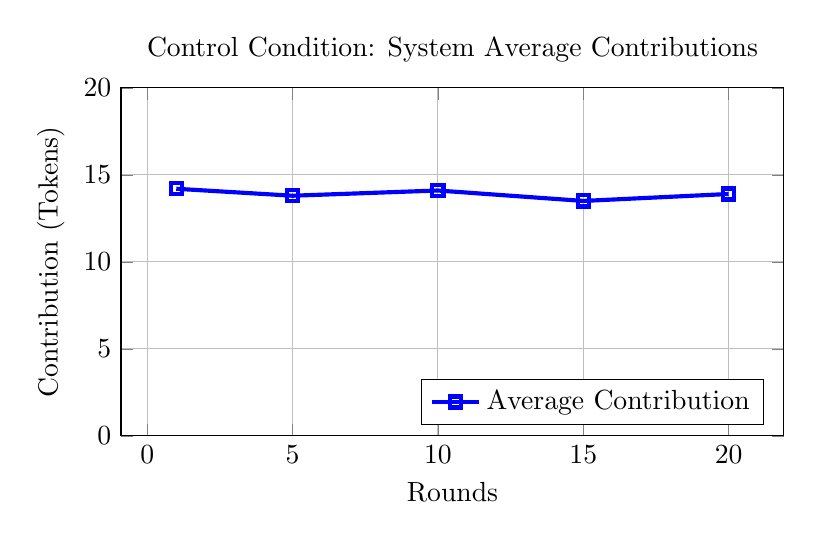
\begin{tikzpicture}
\begin{axis}[
    title={Control Condition: System Average Contributions},
    xlabel={Rounds},
    ylabel={Contribution (Tokens)},
    ymin=0, ymax=20,
    width=10cm, height=6cm,
    grid=major,
    legend pos=south east
]
\addplot[color=blue,mark=square,line width=1.5pt] coordinates {
    (1,14.2) (5,13.8) (10,14.1) (15,13.5) (20,13.9)
};
\addlegendentry{Average Contribution}
\end{axis}
\end{tikzpicture}
\caption{Contributions in the Control condition average ~13.96, showing that agents establish a moderate baseline of cooperation even without reputation systems.}
\end{figure}

\section{Baseline Run 2: The Reputation Mechanism}
\textbf{Setup:} Control setup + continuously updated Reputation Scores (0 to 10) calculated via an Exponential Moving Average (EMA) and broadcasted publicly.

\subsection{Reputation as a Coordination Anchor}
The introduction of numerical reputation scores profoundly alters group dynamics. The EMA algorithm ensures that reputation is slow to build but quick to drop if defection occurs. Agents with high reputations (9.0--10.0) become behavioural anchors. The transparency of reputation creates social proof, prompting 6 out of 7 agents to migrate to SI by round 5, assuming that observing high-reputation peers guarantees a safe institutional environment.

\subsection{The Psychology of Public Scores}
The presence of public scores shifts the agents' internal narratives. In their \texttt{belief\_state}, agents frequently cite maintaining their reputation as a primary objective, overriding raw profit maximization. The numerical anchor provides a heuristic that simplifies the complex social environment, but it also creates blind spots.

\subsection{Interesting Findings}
\textbf{1. The Disconnect Between Reputation and Institution:}
Counterintuitively, the agent with the highest reputation does not reside in the Strict Institution. Agent 5 ends the simulation in SFI with a perfect reputation of 10.0 and wealth of 1,354. They achieved this by contributing 18--20 tokens per round voluntarily. This grounded data point demonstrates that reputation evaluates raw cooperative behaviour, meaning an agent can build immense social capital without exposing themselves to SI's enforcement risks.

\textbf{2. Regressive Enforcement and Wealth Collapse:}
Despite high SI participation, the punishment mechanism proves structurally inequitable for developing agents with low contribution capacities (0.1 multiplier). 
Agent 2 (developing) contributes 10 tokens (their maximum comfortable capacity) but is brutally punished by developed peers who expect absolute contributions to be higher. By round 20, Agent 2 accumulates $-75$ tokens in Stage 2 punishments, causing their cumulative wealth to collapse to \textbf{511 tokens} (down from a starting wealth of 700). Conversely, Agent 4 (developed) contributes similarly but suffers fewer penalties, ending with \textbf{1,770 tokens}.

\begin{table}[H]
\centering
\begin{tabular}{@{}llccc@{}}
\toprule
\textbf{Agent} & \textbf{Group} & \textbf{Final Contribution} & \textbf{Stage 2 Payoff (R20)} & \textbf{Cumul. Wealth (R20)} \\ \midrule
Agent 2 & Developing & 10 & -75 & 511.29 \\
Agent 1 & Developing & 12 & -96 & 933.29 \\
Agent 4 & Developed & 10 & -48 & 1770.09 \\
Agent 6 & Developed & 15 & +2 & 1669.02 \\ \bottomrule
\end{tabular}
\caption{Final round (20) disparities in the Reputation condition highlighting regressive punishment.}
\end{table}

\section{Baseline Run 3: The Voting Condition}
\textbf{Setup:} LLM agents + Voting mechanism. No dynamic reputation (flat 5.0).

\subsection{The Mechanics of Democratic Rule}
The Voting condition allows agents to propose and vote on institutional rules (e.g., minimum contribution thresholds). A rule is enacted if it receives majority support. In theory, this should allow the agents to dynamically adjust the environment to protect themselves. In practice, the absence of reputation scores turns the democratic process into a weapon.

\subsection{The Failure of Voting Without Reputation}
The Voting condition produces the worst collective outcome of any LLM baseline, with an average system wealth of just 1,007. The mechanism reveals that providing agents the ability to vote on rules without providing objective metrics of peer reliability (Reputation) creates a paranoid ecosystem.

\subsection{Interesting Findings}
\textbf{1. Paranoia and False Accusations:}
Without numerical reputation scores, voting creates information regarding \textit{preferences} but not \textit{trustworthiness}. The JSON logs reveal agents generating highly suspicious narratives in their belief states. Agent 5 repeatedly notes: \textit{``adjust my strategy to account for Agent 1's continued manipulative behaviour.''} Without empirical reputation to verify this, the gossip and voting mechanisms amplify distrust rather than coordinate cooperation.

\textbf{2. Catastrophic Decline (Agent 2):}
Agent 2 (developing, SI) finishes with a devastating cumulative wealth of \textbf{16.5}. They experience Stage 2 losses ranging from -78 to -114 in the final 4 rounds alone. Their internal reasoning reflects profound cognitive dissonance under pressure: \textit{``Adjust contribution level downward... Consider increasing my own contribution to SI to encourage others.''} The simultaneous rationalisation of both retreat and escalation highlights how an LLM's strategic reasoning fractures when subjected to continuous, unexplained systemic punishment.

\textbf{3. The Defector's Premium:}
While SI members destroy each other's wealth via voting factionalism and punishment, Agent 0 (developing) switches to SFI from round 6 onward, contributing 20 tokens per round without any punishment exposure. They end with a wealth of 1,278, significantly out-earning all their developing-country peers in SI, perfectly illustrating the institutional exit problem.

\section{Baseline Run 4: Full Condition (All Mechanisms)}
\textbf{Setup:} All mechanisms active (Reputation, Voting, Enhanced Enforcement, Gossip).

\subsection{Systemic Interaction of Mechanisms}
The Full condition tests whether layering multiple cooperative mechanisms creates a robust institution or causes systemic failure through over-engineering. The interaction of Gossip (broadcasting ToM failures), Voting (adjusting rules), and Reputation (scoring actions) creates an incredibly high-pressure cognitive environment for the agents.

\subsection{The Voluntary Cooperation Equilibrium}
When all enforcement mechanisms are maximized, an unexpected equilibrium emerges. By round 13, the majority of the population (Agents 1, 2, 5, 6) flees the Strict Institution (SI) and settles in the Sanction-Free Institution (SFI). 

\subsection{Interesting Findings}
\textbf{1. The SFI-Majority Paradox:}
The agents migrating to SFI are not free-riders. They consistently contribute 14--20 tokens per round. Because they possess high reputations, they realize they do not need the threat of SI punishment to enforce their own cooperation. The data indicates that SFI + high contribution = high reputation + zero punishment risk. By layering all mechanisms, the system paradoxically proves that formal enforcement is redundant when social reputation is sufficiently strong.

\textbf{2. False-Defector Attribution:}
The agents left behind in SI (Agents 0, 3, 4) fall into a trap of false attribution. Agent 0 consistently receives -39 to -73 in punishments, while explicitly blaming Agent 3: \textit{``Given Agent 3's continued free-riding behavior, I plan to introduce a more stringent punishment mechanism...''} The raw data reveals Agent 3 was actively contributing 10 tokens. When subjected to maximum enforcement algorithms, agents blame innocent peers for systemic poor outcomes they cannot accurately trace.

\section{Baseline Runs 5 \& 6: Non-LLM Counterfactuals}

To contextualize the LLM behaviours, two counterfactual runs were executed replacing the LLMs with hardcoded heuristic logic.

\subsection{Baseline\_Random: Noise Injection}
With a purely random strategy, the system experiences high volatility (39 institution switches vs. ~20 in LLM runs). 
\textbf{Interesting Finding (Parsing Failures as Noise):} The random strategy intentionally outputs erratic strings, leading to approximately 20 parser fallback events. Despite this noise, random agents mathematically average a 9.01 token contribution, achieving a collective payoff of 1,190. This is only marginally worse than the Control condition (1,219), suggesting that the uncoordinated punishment friction in pure LLM systems suppresses their theoretical cooperative advantage to near-random levels.

\subsection{Baseline\_Greedy: The Dominant Equilibrium}
All 7 agents are hardcoded to choose SFI and contribute 0 tokens (using the `LLM Greedy Persona`). 
\textbf{Interesting Finding (The Rationality of Defection):} 
There are exactly zero institution switches across the 20 rounds. With no contributions, average final wealth peaks at \textbf{1,360 tokens}—the highest of any 20-round run. Because there are no exogenous climate shocks in this baseline, there is no penalty for failing to provide the public good. Every agent keeps their endowment and receives the base SFI subsidy. This empirically proves that without climate risk, defection is the strictly dominant, mathematically optimal strategy. 

\section{Baseline Runs 7 \& 8: Mixed Populations}

These runs test how sophisticated LLM agents handle explicit bad actors by placing 5 standard LLMs in an environment with 2 hardcoded Greedy agents.

\subsection{LLMs vs. Greedy Agents (30 Rounds)}
In a population of 5 LLMs and 2 Greedy agents, the Greedy agents (Agents 4 and 6) accumulate over 2,100 wealth by round 30 by permanently free-riding in SFI. The extended 30-round duration allows us to observe long-term adaptation.

\subsection{Interesting Findings}
\textbf{1. The Identification-Sanctioning Disconnect:}
The LLM agents successfully identify the Greedy exploiters early in the simulation. Agent 1 notes in round 7: \textit{``...consider reducing my contribution if Agent 4 and Agent 6 continue their opportunistic behavior.''} The ToM scores and Gossip modules function perfectly to label Agents 4 and 6 as defectors. However, because the Greedy agents refuse to leave SFI, the LLMs possess no mechanical means to sanction them. 

\textbf{2. The Closed SI Economy:}
Unable to punish the defectors, the LLMs escalate their own contributions within SI (rising from 15 tokens to 25+ in the final rounds) to capture internal enforcement rewards. They effectively create a closed cooperative economy, abandoning attempts to coerce the SFI free-riders, who subsequently achieve the highest individual payoffs in the entire simulation suite.

\section{Cross-Condition Synthesis and Thesis Implications}

\subsection{The Invariance of Structural Inequality}
No institutional mechanism tested in these baselines successfully closed the wealth gap between developed and developing nations. Across all runs:
\begin{itemize}
    \item Developed agents start at 1,300 and end at 1,300--1,800.
    \item Developing agents start at 700 and end at 500--1,200.
\end{itemize}
SI enforcement is structurally regressive. It punishes low-capacity developing agents for absolute contribution shortfalls. The agents' cognitive architecture (specifically the prompt limitations) prevents them from naturally internalizing proportional capacity scaling when evaluating fairness. This confirms that institutional design alone cannot resolve systemic inequality without explicit redistributive algorithms like the Loss \& Damage Fund.

\subsection{The Cognitive Limits of LLM Agents in Game Theory}
The baseline studies reveal critical limits in LLM strategic play:
\begin{itemize}
    \item \textbf{The Reasoning-Action Gap:} LLMs frequently generate mathematically optimal plans in text but fail to execute them in numerical output.
    \item \textbf{Punishment Myopia:} LLMs deploy punishment reactively rather than strategically, failing to use sanctions as a forward-looking deterrent.
    \item \textbf{Information Overload:} When Voting, Reputation, and Gossip are combined, LLM strategic performance deteriorates due to the complexity of the context window.
\end{itemize}

\subsection{Thesis Conclusion: The Necessity of Climate Risk}
The baseline data conclusively supports the central premise of the thesis: endogenous cooperative institutions require existential risk to function optimally. In these shock-free environments:
1. The Greedy defection strategy yields the absolute highest individual payoffs, proving that cooperation without risk is economically irrational.
2. The Voting mechanism collapses into paranoia due to the lack of objective anchors.
3. Over-enforcement causes a flight to Sanction-Free Institutions, rendering the Strict Institution obsolete.
4. Inequality persists and compounds regardless of the cooperative mechanism.

It is only through the introduction of exogenous Climate Shocks and the redistributive necessity of the Loss \& Damage Fund (LDF) that cooperation transforms from an irrational, intrinsic LLM bias into a mathematically dominant survival imperative.

\end{document}
